%paper prototype

\section{paper prototype}

\subsection{preparement}

After choosing our idea, we build a paper prototype for it. The prototype should help us to find a basic structure of our GUI
before starting the real implementation. We sketched our views, a Web-Version and a android version. After many new tries we
obtained our final version. We digitalized the results without any color.

\begin{figure}[!h]
	\begin{subfigure}[b]{0.5\textwidth}
		\centering
		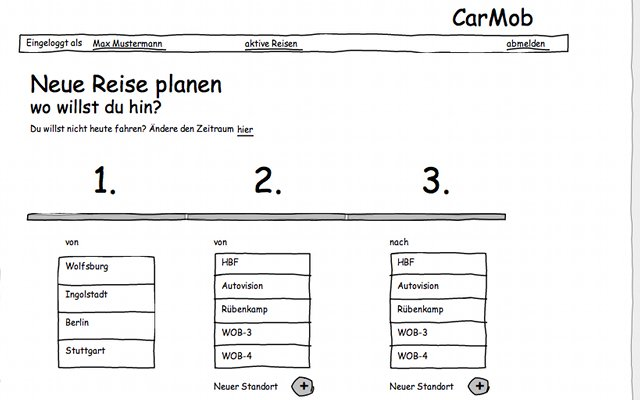
\includegraphics[width=\textwidth]{images/Web_1.jpg}
		\caption{searching a tour}
		\label{fig:web1}
	\end{subfigure}
	\begin{subfigure}[b]{0.5\textwidth}
		\centering
		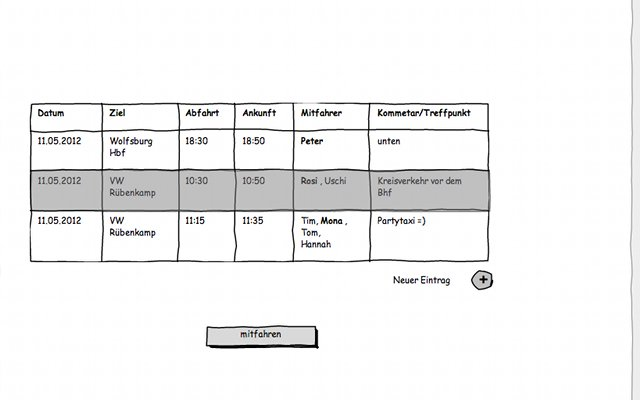
\includegraphics[width=\textwidth]{images/Web_2.jpg}
		\caption{choose a tour}
		\label{fig:web2}
	\end{subfigure}
	\caption{paper prototype: Web}
	\label{fig:web}
\end{figure}

\begin{figure}[!h]
	\begin{subfigure}[b]{0.3\textwidth}
		\centering
		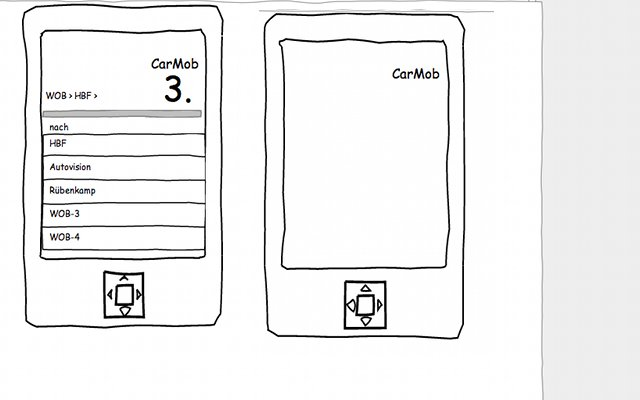
\includegraphics[width=\textwidth]{images/App_4.jpg}
		\caption{searching a tour}
		\label{fig:app1}
	\end{subfigure}
	\begin{subfigure}[b]{0.3\textwidth}
		\centering
		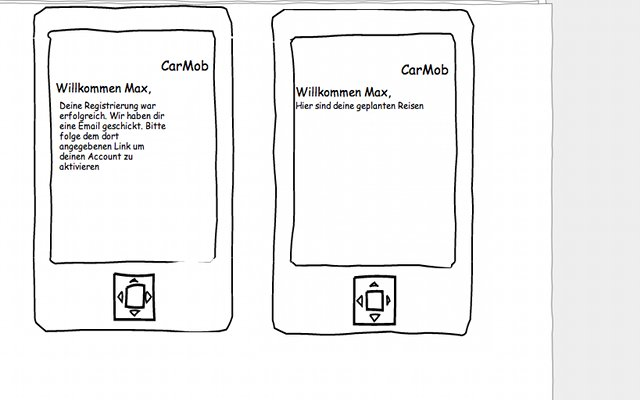
\includegraphics[width=\textwidth]{images/App_2.jpg}
		\caption{choose a tour}
		\label{fig:app2}
	\end{subfigure}
		\begin{subfigure}[b]{0.3\textwidth}
		\centering
		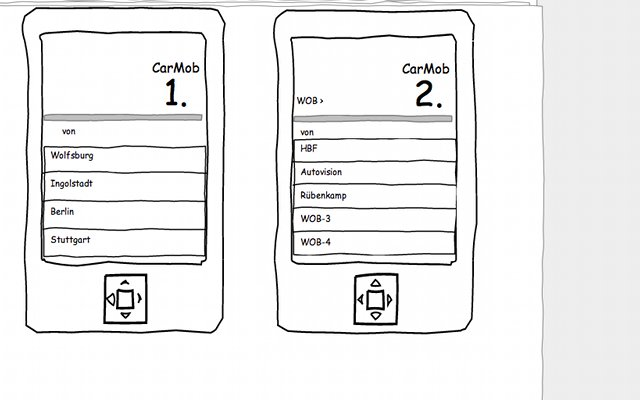
\includegraphics[width=\textwidth]{images/App_3.jpg}
		\caption{choose a tour}
		\label{fig:app3}
	\end{subfigure}
	\caption{paper prototype: App}
	\label{fig:app}
\end{figure}

\clearpage

\subsection{implementation}

During the tests it became clear, that nobody know why 'active tours' means. For us it was a totally easy term. We found a lot of
these misconceptions. But also semantic failures were offered. All things considered these tests helped us a lot. And the best was
they didn't take much time.


